% ================================================================
% Rotatable Networks. JASA (Theory & Methods) submission draft.
% Compile: pdflatex main -> bibtex main -> pdflatex main x2,
% then compile supplement.tex the same way (it reads main.aux via xr).
% Set \blind to 1 for the review version, 0 for the unblinded version.
% At template adoption, switch to the ASA/Taylor & Francis class and its
% agsm-style .bst (not installed in this build environment; apalike is
% the stand-in author-year style until then).
% ================================================================
\documentclass[12pt]{article}
\newcommand{\blind}{1}

\usepackage[margin=1in]{geometry}
\usepackage{amsmath,amssymb,amsthm,mathtools}
\usepackage{bm}
\usepackage{graphicx}
\usepackage{booktabs}
\usepackage[protrusion=true,expansion=false]{microtype}
\usepackage[round]{natbib}
\usepackage{setspace}
\usepackage{caption}
\usepackage{enumitem}
\usepackage{xcolor}
\definecolor{linkink}{RGB}{28,60,120}
\usepackage[colorlinks=true,linkcolor=linkink,citecolor=linkink,urlcolor=linkink]{hyperref}
\captionsetup{font={small,stretch=1.05},labelfont=bf}

\doublespacing

% ================================================================
\newtheorem{theorem}{Theorem}
\newtheorem{proposition}{Proposition}
\newtheorem{corollary}{Corollary}
\newtheorem{lemma}{Lemma}
\newtheorem{conjecture}{Conjecture}
\theoremstyle{definition}
\newtheorem{definition}{Definition}
\newtheorem{example}{Example}
\theoremstyle{remark}
\newtheorem{remark}{Remark}

% ================================================================
\newcommand{\R}{\mathbb{R}}
\newcommand{\N}{\mathbb{N}}
\newcommand{\E}{\mathbb{E}}
\newcommand{\Prob}{\mathbb{P}}
\newcommand{\OO}{\mathbb{O}}
\newcommand{\eqd}{\overset{d}{=}}
\newcommand{\tod}{\overset{d}{\to}}
\newcommand{\toas}{\overset{\mathrm{a.s.}}{\to}}
\newcommand{\toP}{\overset{P}{\to}}
\newcommand{\iid}{\overset{\mathrm{iid}}{\sim}}
\newcommand{\Sym}{\mathrm{Sym}}
\newcommand{\tr}{\operatorname{tr}}
\newcommand{\diag}{\operatorname{diag}}
\newcommand{\spec}{\operatorname{spec}}
\newcommand{\hollow}{\operatorname{hollow}}
\newcommand{\Haar}{\mathrm{Haar}}
\newcommand{\GOE}{\mathrm{GOE}}
\newcommand{\SaS}{\mathrm{S}\alpha\mathrm{S}}
\newcommand{\lam}{\lambda}
\newcommand{\blam}{\bm{\lambda}}
\newcommand{\bgam}{\bm{\gamma}}
\DeclareMathOperator*{\argmax}{arg\,max}

\title{\bfseries Rotatable Networks}

\ifnum\blind=1
\author{Author names blinded for review}
\else
\author{[Author names]\thanks{[Affiliations, ORCID, correspondence,
and funding; complete before unblinded submission.]}}
\fi

\date{}

\begin{document}
\maketitle

\begin{abstract}
Weighted networks (brain connectivity matrices, stock correlation
matrices, traffic flows) are usually summarized by a handful of
statistics such as clustering or modularity and judged against an
informal null model. We study the consequences of one symmetry: a
random network is rotatable if its distribution is unchanged by
rotations of the underlying coordinate system. The rotatable network
models that stay consistent as nodes are added are exactly mixtures of
spiked Gaussian orthogonal ensembles, an isotropic form of the
low-rank-plus-noise models assumed in practice; the theory covers
dense real-weighted networks and excludes sparse binary graphs.
Within any such model the eigenvalues carry all the information: given
the eigenvalues, the network is a uniformly random rotation. This
yields a Monte Carlo test of the symmetry, exact for fully observed
matrices and with a quantified size bound for zero-diagonal data, and
a conditional residual for every network statistic. An extension
covers heavy-tailed networks. On a human connectome, stock
correlations, and air traffic, eigenvalue reconstruction is high for
clustering, modularity, and kurtosis, while localization and strength
heterogeneity carry the conditional signal, attributed to named nodes
with exact familywise control.
\end{abstract}

\noindent{\bfseries Keywords:} exchangeable arrays; Haar measure;
randomization inference; spiked random matrices; graphon; stable
distributions

\newpage

\section{Introduction}\label{sec:intro}

Many scientific fields analyze data in the form of a real symmetric
weighted network on $n$ nodes. Network neuroscience studies functional
connectomes, matrices of correlations between the activity of brain
regions \citep{bullmore2009complex,rubinov2010complex}; genomics studies
gene co-expression networks \citep{zhang2005general}; empirical finance
studies correlation matrices of asset returns
\citep{laloux1999noise,plerou2002random}. Standard practice computes scalar summaries, weighted clustering,
modularity, path length, strength heterogeneity, and interprets them
against a null ensemble. The stated model is almost always ``low-rank
signal plus rotation-invariant noise,'' analyzed with spiked random
matrix theory
\citep{johnstone2001distribution,baik2005phase,benaych2011eigenvalues};
the low-rank structure is a modeling choice, motivated by empirical
spectra and imposed without derivation. The nonparametric alternative,
exchangeable network theory, represents any weighted network with
exchangeable node labels by a bivariate graphon
\citep{aldous1981representations,hoover1979relations}, but the graphon
is difficult to estimate even for binary graphs
\citep{wolfe2013nonparametric,gao2015rate,klopp2017oracle} and supplies
no finite-sample null distribution for the summaries practitioners
report.

Three questions arise. Is there a symmetry assumption
under which the model class used in practice is forced by first
principles? Under that model class, which network statistics carry
information beyond the eigenvalues of the observed matrix? And can
departures from the symmetry be tested exactly, at finite $n$, without
estimating parameters or choosing a generative null?

This paper answers the three questions by strengthening the symmetry
that underlies exchangeable network theory. Node labels in a weighted
network are arbitrary, and in the applications above something more is
arbitrary as well: a correlation network is computed from node-level
signals whose coordinate system is a convention, and the natural
invariance for such data is invariance under rotation of the node space
in addition to relabeling. We therefore study jointly rotatable arrays,
random symmetric $X$ with
\begin{equation}\label{eq:rotdef}
U X U^{\top} \eqd X \quad\text{for every finite orthogonal } U,
\end{equation}
a notion whose probabilistic theory is due to
\citet{freedman1962invariants,dawid1977,aldous1981representations} and
\citet{kallenberg1995multivariate,kallenberg2005probabilistic}. Two facts motivate \eqref{eq:rotdef} here. If $X = h(Y^{\top}Y)$ for a
$T\times n$ panel $Y$ of node-level signals that are jointly Gaussian
with an isotropic prior on loading directions, and $h$ is
conjugation-equivariant ($h(UGU^\top)=Uh(G)U^\top$; the identity or
any spectral function), then $YU^{\top}\eqd Y$ and hence
$UXU^{\top}\eqd X$: rotatability is inherited from isotropy of the
latent coordinate system. Entrywise transforms such as Fisher-$z$ are
not equivariant; they enter through the preprocessing clause of
Proposition~\ref{prop:robust}, not through this inheritance. And any analysis that models a network as signal plus
rotation-invariant noise has already assumed \eqref{eq:rotdef} for the
noise; we impose the symmetry on the whole object. The invariance acts
on the latent coordinate system that generates the data, the named
nodes are never claimed interchangeable, and rotatability functions
throughout as a sharp reference null. The cost of the stronger
symmetry is support: rotatable laws have Gaussian ergodic components, so
the theory covers dense real-valued networks and excludes sparse binary
graphs.

Combining \eqref{eq:rotdef} with sampling consistency, the requirement
that the model does not change when one more node is observed,
characterizes the model class: a network model is orthogonally
invariant and sampling-consistent if and only if it is a mixture of
spiked Gaussian orthogonal ensembles (Theorem~\ref{thm:rep}). The probabilistic core, including the symmetric case, is the
representation theory of
\citet{kallenberg1988some,kallenberg1995multivariate,kallenberg2005probabilistic};
the characterization of sampling-consistent network models, and the
statistical program built on it, are, to our knowledge, new. The bivariate graphon reduces, under the stronger symmetry, to a
noise level $\sigma$ and a square-summable eigenvalue sequence
$\blam$, and the relevant moments reduce to cycles: cycle expectations
equal power sums of $\blam$, tree expectations vanish, and a product formula holds for vertex-disjoint unions of
cycles (Proposition~S1 in the Supplement), giving identifiability and a
method of moments.

Three statistical consequences follow. Under any rotatable model the
ordered spectrum of the observed network is sufficient, and
conditionally on the spectrum the network is a Haar-random rotation of
it, for every value of the parameter (Theorem~\ref{thm:suff}); the
conditional distribution of any non-spectral statistic given the
eigenvalues is therefore parameter-free (Corollary~S1 in the
Supplement). The conditional representation yields a finite-sample Monte Carlo
test of rotatability, re-rotating the observed spectrum and
recomputing any battery of statistics (Theorem~\ref{thm:test}): no
parameters are estimated, the composite null is covered, calibration holds for any observed spectral shape and is exact when
the full matrix is observed; against the same rotatable truth, a weight-permutation null, which calibrates a different hypothesis,
rejects $51\%$ of the time (Section~\ref{sec:exp-test}).
Constrained observations, hollow or unit-diagonal, are outside the
total-variation route by a mutual-singularity obstruction (Supplement,
Remark~S1); the pipeline's guarantee is instead statistic-level, with
an explicit concentration modulus and rate
$n^{-1/4}(\log n)^{1/2}$ (Proposition~\ref{prop:hollowrate}), and
size is measured in Section~\ref{sec:experiments}. Consistency holds
against localized alternatives such as hubs and modules
(Proposition~S3), with the exact-null status of spherical spikes and the consistency
threshold recorded in Corollary~S2. The same draws produce, for each statistic, a conditional residual,
the difference between the observed value and its Haar-conditional
expectation given the spectrum, proposed as the standard output: it
quantifies exactly the part of each summary that the eigenvalues do
not determine.
And embedding the ergodic law in growing corners shows that the
Baik--Ben~Arous--P\'ech\'e transition
\citep{baik2005phase,feral2007largest,benaych2011eigenvalues} describes
the finite-$n$ resolution of a fixed infinite network, with effective
spikes $\sqrt{n}\,\lam_k/\sigma$, an $n^{-1/2}$ detection boundary, and
consistent plug-in estimation above it (Proposition~S2).

A secondary contribution extends the symmetry beyond the Gaussian case.
Replacing the rotation group by the symmetry that characterizes
$\ell_p$, $p\in(0,2)$, in the sense of matched-norm quadratic forms, we
construct spiked symmetric $p$-stable ensembles, prove that they are
$p$-rotatable, and show that the invariance forces a canonical
diagonal-to-off-diagonal scale ratio $2^{(p-1)/p}$
(Theorem~\ref{thm:stable}); completeness at the array level is open
(Conjecture~\ref{conj:stable}). With no $p$-analogue of the Haar frame
there is no exact conditional test at $p<2$; as a surrogate we test
rotatability of the normal-scores transform, which separates marginal,
tail-driven departures from persistent eigenvector localization
(Section~\ref{sec:diagnostic}).

Rotatability is proposed as a sharp null hypothesis; its value lies
in what a rejection localizes. Anatomical, sector, and geographic structure are expected departures
in brains, markets, and traffic, and the real-data analyses reject
strict rotatability through exactly the statistics the theory predicts
must carry such violations; the
scientific output is the direction of rejection and the conditional
residuals. On the data of
Section~\ref{sec:experiments}, several routinely tabulated summaries
are close to their Haar-conditional expectations, while eigenvector
localization carries the non-spectral signal.

\subsection{Contributions}

\begin{enumerate}[leftmargin=1.7em,itemsep=0.1em]
\item \emph{Characterization} (Section~\ref{sec:representation}).
Theorem~\ref{thm:rep}: a weighted network model is orthogonally
invariant and sampling-consistent if and only if it is a mixture of
spiked Gaussian orthogonal ensembles, with unique mixing measure over
$(\rho,\sigma,\blam)\in\R\times\R_{+}\times\ell_{2,*}$; cycle moments
identify $(\sigma,\blam)$ (Proposition~S1).
\item \emph{Exact conditional inference} (Sections~\ref{sec:sufficiency}
and \ref{sec:test}). Theorem~\ref{thm:suff}: the spectrum is sufficient
with Haar conditionals, for every rotatable model, so non-spectral
summaries are conditionally parameter-free (Corollary~S1).
Theorem~\ref{thm:test}: an exact finite-sample Monte Carlo test of the
composite null, estimating no parameters, calibrated for any observed
spectrum, reported with conditional residuals
(Definition~\ref{def:residual}).
\item \emph{Guarantees and calibration}. Size at most
$\alpha+\varepsilon$ under $\varepsilon$-approximate rotatability of
the fully observed matrix, with a preprocessing clause and a
bounded-loss risk bound (Proposition~\ref{prop:robust}); a
statistic-level size guarantee for the zero-completion pipeline with
concentration modulus and rate $n^{-1/4}(\log n)^{1/2}$
(Proposition~\ref{prop:hollowrate}); nodewise attribution with exact
familywise control (Sections~\ref{sec:test}
and~\ref{sec:exp-nodewise}); consistency
against supercritical localized spikes (Proposition~S3); the
Baik--Ben~Arous--P\'ech\'e transition as the resolution limit of a
fixed network, with consistent plug-in estimation (Proposition~S2);
empirical size checks for the hollow and finite-$T$ correlation
pipelines (Section~\ref{sec:experiments}).
\item \emph{Heavy tails and experiments} (Sections~\ref{sec:lp} and
\ref{sec:experiments}). Spiked symmetric $p$-stable ensembles are
$p$-rotatable with a canonical diagonal (Theorem~\ref{thm:stable});
completeness is Conjecture~\ref{conj:stable}; a Gaussianization
diagnostic with explicit surrogate status; analyses of a human
connectome, S\&P~500 correlation networks, an air-traffic network, and
a synthetic cohort study, labeled as such, with released code and fixed
seeds.
\end{enumerate}

Sections~\ref{sec:setup}--\ref{sec:experiments} develop the setup,
the characterization, sufficiency and the exact test, heavy tails, and
the experiments; the Supplement contains all proofs and deferred
statements.

\subsection{Related work}\label{sec:related}

Exchangeable arrays and graph limits are surveyed by
\citet{austin2008exchangeable,orbanz2015bayesian,lovasz2012large}
(sparse extensions:
\citealp{caron2017sparse,borgs2019lp}); rotatable arrays are due to
\citet{aldous1981representations,kallenberg1988some,kallenberg1995multivariate},
synthesized in \citet[Chapter~8]{kallenberg2005probabilistic}, with
antecedents \citep{freedman1962invariants,dawid1977,schoenberg1938,vershik2002}. The nearest
statistical relative is the Dovbysh--Sudakov representation of
exchangeable positive semidefinite arrays, structural in spin glasses
\citep{dovbysh1982gram,panchenko2013sherrington} but not, to our
knowledge, used as a data model; we could locate no application of
rotatable arrays to network data. Spiked models, the BBP transition, shrinkage, detection limits, and
delocalization:
\citet{johnstone2001distribution,baik2005phase,feral2007largest,capitaine2009largest,benaych2011eigenvalues,bai2008central,donoho2018optimal,onatski2013asymptotic,perry2018optimality,orourke2016eigenvectors}.
Network-neuroscience summaries and null models:
\citet{bullmore2009complex,rubinov2010complex,vasa2022null}; weighted
clustering \citep{onnela2005intensity}; modularity \citep{newman2006}.
Financial correlation matrices:
\citet{laloux1999noise,plerou2002random,bouchaud2009}. Stable laws and
$L^p$-symmetric sequences:
\citet{bretagnolle1966lois,cambanis1983alpha,samorodnitsky1994stable}.
Rotation tests based on random orthogonal transformations exist in
multivariate analysis \citep{langsrud2005rotation,perry2010rotation};
Theorem~\ref{thm:test} differs in conditioning on the observed
spectrum, which fixes the reference distribution for the whole
composite class. General theory for group-invariance randomization
covers validity and power for compact groups
\citep{dobriban2022consistency,koning2024more}; Theorem~\ref{thm:test}
is its $\OO(n)$-orbit instantiation with the spectrum as maximal
invariant, and the network content of the paper lies in
Theorems~\ref{thm:rep} and \ref{thm:suff} and the residual protocol.
Theorem~\ref{thm:rep} identifies the ergodic class with the eigenmodel
of \citet{hoff2008eigenmodel} under isotropic Gaussian latent
positions, a first-principles derivation of a model already in
statistical use. Our sufficiency and testing arguments otherwise use
classical invariance tools \citep{eaton1989group,lehmann2005testing},
and the exactness of Monte Carlo randomization tests goes back to
\citet{dwass1957}; see \citet{hemerik2018exact}. Eigenvector randomization heuristics
circulate in network neuroscience \citep{vasa2022null};
Theorem~\ref{thm:test} identifies the hypothesis such procedures test
and supplies exact level, and Corollary~S1 characterizes what they
cannot detect.

\subsection{Notation}\label{sec:notation}

$\Sym_n$ is the space of real symmetric $n\times n$ matrices and
$\OO(n)$ the orthogonal group with Haar probability measure $\Haar_n$.
For an infinite symmetric array $X=(X_{ij})_{i,j\in\N}$, $X_n$ denotes
its leading principal $n\times n$ submatrix (its corner). A network is
a hollow symmetric array (zero diagonal), the diagonal being unobserved
or conventionally zero; $\hollow(A)$ zeroes the diagonal of $A$. $W$
denotes a symmetric array with independent entries $W_{ij}\sim N(0,1)$
for $i<j$ and $W_{ii}\sim N(0,2)$ (the infinite GOE pattern), and
$\GOE(n)$ its $n\times n$ corner. For $\blam=(\lam_k)\in\ell_2$ we
write $p_m(\blam)=\sum_k\lam_k^m$, $m\ge 2$. $\Delta_n:=\{d\in\R^n:d_1\ge\cdots\ge d_n\}$ collects ordered
vectors, and $D(A)\in\Delta_n$ is the
vector of eigenvalues of $A\in\Sym_n$ in decreasing order; on the event
of simple spectrum, $V(A)\in\OO(n)$ is the eigenvector matrix with the
sign convention that the largest-magnitude entry of each column is
positive, so $A=V\diag(D)V^{\top}$. Localization statistics use the
$K_{\mathrm{loc}}=10$ eigenpairs with the largest absolute eigenvalues;
this ordering is used only there and is stated where it applies. The
effective spike of $\lam_k$ at sample size $n$ is
$s_k=\sqrt{n}\,\lam_k/\sigma$. All proofs are in the Supplement.

\section{From exchangeability to rotatability}
\label{sec:setup}

\subsection{Two symmetries}

Let $X=(X_{ij})_{i,j\in\N}$ be a random element of $\Sym_\infty$, the
symmetric real arrays. Exchangeability is invariance under the permutation
action $(\pi\cdot X)_{ij}=X_{\pi(i)\pi(j)}$ for finite permutations $\pi$.
The Aldous--Hoover theorem represents every such array as
$X_{ij}=f(\alpha,U_i,U_j,\varepsilon_{ij})$ with i.i.d.\ uniform latent
variables; the ergodic components are indexed by the measurable kernel $f$, a
weighted graphon with edge noise
\citep{aldous1981representations,hoover1979relations}.

Rotatability replaces the countable permutation group by the larger
finitary orthogonal group. Embed $U\in\OO(n)$ into the infinite orthogonal matrices
fixing all coordinates beyond $n$, $\tilde U=U\oplus I$.

\begin{definition}[Joint rotatability]
\label{def:rot}
$X$ is \emph{jointly rotatable} if $\tilde U X \tilde U^\top \eqd X$ for
every $n$ and every $U\in\OO(n)$.
\end{definition}

Permutation matrices are orthogonal, so a jointly rotatable array is
exchangeable: rotatability is a submodel of the graphon class, and
Section~\ref{sec:test} tests the submodel within the model. The
qualifier \emph{joint} distinguishes \eqref{eq:rotdef} from
\emph{separate} rotatability for rectangular arrays
\citep{aldous1981representations}; symmetric networks require the
joint action. The cost of the stronger symmetry is support, Gaussian
ergodic components (Theorem~\ref{thm:rep}), so binary graphs are
outside the theory and the intended scope is dense real-weighted
networks.

\subsection{Sampling consistency}
\label{sec:consistency}

A statistical model for networks is a family $\{P_n\}_{n\ge1}$, $P_n$ a law
on $\Sym_n$, describing data observed on $n$ nodes. Two closure properties
are natural.

\begin{definition}
\label{def:consistent}
$\{P_n\}$ is \emph{orthogonally invariant} if $X\sim P_n$ implies
$UXU^\top\sim P_n$ for all $U\in\OO(n)$. It is \emph{sampling-consistent}
if the leading $(n-1)\times(n-1)$ corner of $X\sim P_n$ has law $P_{n-1}$.
\end{definition}

Sampling consistency is the projectivity requirement underlying exchangeable
network theory \citep{orbanz2015bayesian}: the model must not change when one
more node is observed. Finite invariance alone does not restrict the
spectral law: for fixed $n$, orthogonal invariance says only that
$X = U D U^\top$ with $U$ Haar distributed and independent of the
eigenvalues $D$, and any law for $D$ qualifies. The next section shows that
adding sampling consistency reduces this class to mixtures of spiked
Gaussian ensembles.

The extension step, that $\{P_n\}$ is orthogonally invariant and
sampling-consistent if and only if it is the family of corner laws of
one jointly rotatable array with a unique law, is part of
Theorem~\ref{thm:rep} below. For parameter identification we fix the
canonical order on spike sequences: $a\succeq_*b$ if $|a|>|b|$, or
$|a|=|b|$ and $a\ge b$, and $\ell_{2,*}$ is the set of
$\blam\in\ell_2$ with $\lam_k\succeq_*\lam_{k+1}$ for every $k$; each
signed multiset of nonzero square-summable coefficients has exactly
one representative in $\ell_{2,*}$, zeros appended when finite. For
probability measures on one space,
$d_{\mathrm{TV}}(\mu,\eta):=\sup_A|\mu(A)-\eta(A)|$, and for bounded
$g$, $\operatorname{osc}(g):=\sup g-\inf g$.

\section{Representation, identifiability, and finite-$n$ calibration}
\label{sec:representation}

\subsection{The characterization}

The following theorem is the foundation of the paper. The
representation, including the symmetric case, is due to
\citet{kallenberg1988some,kallenberg1995multivariate}, as synthesized
in \citet[Chapter~8]{kallenberg2005probabilistic}; our contribution is the packaging as a statistical model class, the
equivalence with orthogonal invariance plus sampling consistency for
network models, now internal to the theorem, and the statistical
program built on the class. The Supplement proves the theorem in full
from \citet[Theorem~5.1]{kallenberg1988some}, including uniqueness of
the mixing measure, measurability of the parameterization, and
almost-sure convergence simultaneous over all entries. Throughout,
$W$ denotes a symmetric array with $W_{ij}\sim N(0,1)$ for $i<j$,
$W_{ii}\sim N(0,2)$, independent entries (the infinite GOE pattern), and
$(\xi_{ki})_{k,i\in\N}$ an independent array of i.i.d.\ $N(0,1)$ variables.

\begin{theorem}[Spiked representation of rotatable networks]
\label{thm:rep}
Let $X$ be a random element of $\Sym_\infty$. The following are equivalent.
\begin{enumerate}[label=(\roman*),itemsep=1pt,topsep=2pt]
\item $X$ is jointly rotatable.
\item $X$ is a mixture of \emph{ergodic} laws
$R_{\rho,\sigma,\blam}$, $\rho\in\R$, $\sigma\ge0$,
$\blam=(\lam_k)\in\ell_2$, where under $R_{\rho,\sigma,\blam}$
\begin{equation}
\label{eq:rep}
X_{ij} \;=\; \rho\,\delta_{ij} \;+\; \sigma W_{ij}
\;+\; \sum_{k=1}^{\infty} \lam_k\bigl(\xi_{ki}\xi_{kj}-\delta_{ij}\bigr),
\end{equation}
the series converging almost surely and in $L^2$, simultaneously
over all entries.
\end{enumerate}
With $\blam$ in the canonically ordered space $\ell_{2,*}$ of
Section~\ref{sec:setup}, the mixing measure over
$(\rho,\sigma,\blam)$ is unique, and the $R_{\rho,\sigma,\blam}$ are
exactly the ergodic (extreme) rotatable laws. A network model
$\{P_n\}$ is orthogonally invariant and sampling-consistent if and
only if each $P_n$ is the corner law of one such mixture, with the
same, again unique, mixing measure for every $n$.
\end{theorem}

First, with $\Xi_k=(\xi_{k1},\xi_{k2},\dots)$ the ergodic law is an
infinite-width analogue of $\sigma\,(\text{Wigner noise}) +
\sum_k\lam_k\,\Xi_k\Xi_k^\top$, the low-rank-plus-noise structure
spiked random matrix practice assumes, here the unique class closed
under the two properties of Definition~\ref{def:consistent}; it is the
eigenmodel of \citet{hoff2008eigenmodel} with isotropic Gaussian
latent positions, derived from the symmetry, and the rotational
freedom in the factor index removes any basis choice, making the
spectrum canonical. Second,
$(\sigma,\blam)$ replaces the graphon: a scalar and a point in $\ell_{2,*}$, identified exactly in the
canonical order, with negative $\lam_k$ allowed (disassortative
components); under each ergodic law eigenvector supports are Haar-generic:
privileged node clusters are excluded, low-dimensional signal is kept. Third,
a network observes the hollow part of $X$: $\rho$ is invisible and the
diagonal terms of \eqref{eq:rep} are unobserved. We write $P^{\mathrm{net}}_{\sigma,\blam}$
for the law of the hollow array $(X_{ij})_{i\ne j}$ under
$R_{0,\sigma,\blam}$ and call it the \emph{ergodic rotatable network law}.
For inference we adopt the zero-diagonal completion (a hollow observed
matrix is completed with zeros); Remark~\ref{rem:hollow} in
Section~\ref{sec:test} states the exact scope of the test under this
convention. What the class excludes is equally concrete: the graphon-Gaussian model, $X_{ij}=w(U_i,U_j)$ plus independent
Gaussian noise with nonconstant smooth $w$, degree heterogeneity, localized hubs, and
geometric structure all violate \eqref{eq:rotdef}, and
Section~\ref{sec:test} shows they are detectable.



\subsection{Identifiability and the collapse of moment structure}

For binary exchangeable graphs, the homomorphism densities over all
finite graphs determine the graphon up to equivalence
\citep{lovasz2012large}. Under rotatability the moment structure
collapses to cycles. For distinct indices $i_1,\dots,i_m$ and $m\ge3$,
\begin{equation}
\label{eq:cycles}
\E\bigl[X_{i_1i_2}X_{i_2i_3}\cdots X_{i_mi_1}\bigr] \;=\; p_m(\blam)
\;=\;\sum_k \lam_k^m ,
\qquad
\E\bigl[X_{12}^2\bigr] \;=\; \sigma^2 + p_2(\blam),
\end{equation}
and the expectation of $\prod_{e\in F}X_e$ vanishes whenever some edge
of the finite simple graph $F$ lies in no cycle (in particular for every
tree), while for $F$ a vertex-disjoint union of cycles it equals the
product of the corresponding power sums. The scope is exact: cycles
sharing a vertex and repeated edges generate additional terms, and
Proposition~S1 in the Supplement states the boundary cases. These
identities identify $(\sigma^2,\{\lam_k\})$ from the ergodic law and
give a moment method, empirical cycle averages estimating power sums and
Newton's identities converting power sums to eigenvalues; the spectral
route of the next subsection is more efficient in practice, but
\eqref{eq:cycles} shows the moment information in this graph family is
carried by cycle counts, with the bivariate graphon replaced by one real
sequence.

\subsection{Finite-$n$ calibration}
\label{sec:bbp}

Fix an ergodic law and observe its $n\times n$ corner $X_n$. Normalizing
by $\sqrt n$ puts the noise on the standard Wigner scale:
\[
\frac{X_n}{\sqrt n} \;=\; \frac{\sigma}{\sqrt n} W_n
\;+\;\sum_k \bigl(\sqrt n\,\lam_k\bigr)\,u_k^{(n)}u_k^{(n)\top} + o_P(1),
\qquad u_k^{(n)} = \Xi_k^{(n)}/\lVert\Xi_k^{(n)}\rVert,
\]
so the ergodic component behaves, at sample size $n$, as a spiked Wigner
matrix with effective spikes $s_k=\sqrt n\,\lam_k/\sigma$, and classical
spiked-Wigner asymptotics
\citep{feral2007largest,capitaine2009largest,benaych2011eigenvalues}
transfer directly. Proposition~S2 in the Supplement records the three
consequences the paper uses. Every nonzero $\lam_k$ is eventually
resolved: $\mu_k\toas s_k+1/s_k$ once $s_k>1$, and the number of
eigenvalues of $X_n/(\sigma\sqrt n)$ outside $[-2,2]$ converges a.s.\ to
the number of nonzero spikes. Against local sequences
$\lam^{(n)}=c\,n^{-1/2}$ the boundary is $c=\sigma$: below it the spiked and null sequences are contiguous and no consistent test
exists \citep{onatski2013asymptotic,perry2018optimality};
above it the top eigenvector attains squared overlap $1-c^{-2}\sigma^2$
with the planted factor. And the parameters are estimable by plug-in:
$\hat\sigma$ from the bulk upper quartile, $\hat\lam_k$ from
$\psi^{-1}(\mu_k)$ with $\psi(s)=s+1/s$, and $\hat K$ from the count of
outliers, all strongly consistent. Observing more nodes does not change
the array; it changes which eigenvalues the corner resolves, and the
boundary $\lam\asymp n^{-1/2}$ prices the noise. Above the boundary,
estimation of the ergodic parameter is a sequence problem with parametric
rates, while graphon estimation has nonparametric rates
\citep{gao2015rate,klopp2017oracle}; optimal shrinkage refinements
\citep{donoho2018optimal} apply unchanged.

\section{Spectral sufficiency}
\label{sec:sufficiency}

Fix $n$ and consider the observed matrix $X_n\in\Sym_n$. Recall from
Section~\ref{sec:notation} that $D(X)\in\R^n$ is the vector of eigenvalues
in decreasing order and, on the event of simple spectrum (which has
probability one under every rotatable law with $\sigma>0$), $V(X)\in\OO(n)$
is the sign-normalized eigenvector matrix, so
$X = V\,\diag(D)\,V^\top$.

\begin{theorem}[Spectral sufficiency]
\label{thm:suff}
Let $\mathcal{P}$ be any family of orthogonally invariant laws on
$\Sym_n$, for example the fully observed $n\times n$ corners, diagonal
retained, of the jointly rotatable laws $R_{\rho,\sigma,\blam}$ of
Theorem~\ref{thm:rep} and arbitrary mixtures of them; the hollow laws
$P^{\mathrm{net}}_{\sigma,\blam}$ are not orthogonally invariant
(Remark~\ref{rem:hollow}) and are excluded. Then:
\begin{enumerate}[label=(\roman*),itemsep=1pt,topsep=2pt]
\item For every $P\in\mathcal{P}$, conditionally on $D(X)$ the matrix $X$
is distributed as $U\,\diag(D)\,U^\top$ with $U\sim\Haar_n$
independent of $D$; in particular the conditional law of $X$ given $D$ is
the same for all $P\in\mathcal{P}$.
\item $D(X)$ is sufficient for $\mathcal{P}$ in the strong,
common-kernel sense: one Markov kernel, free of $P$, is a regular
conditional law of $X$ given $D(X)$ under every $P\in\mathcal P$; no
domination assumption on $\mathcal{P}$ is required.
\item On the simple-spectrum event, the frame $V(X)$ follows the
sign-normalized Haar law $\nu_n$, the pushforward of
$\Haar_n$ under columnwise sign normalization, which is not
Haar measure on $\OO(n)$, independently of $D(X)$ and identically for
every $P\in\mathcal{P}$: the frame is an ancillary complement to the
spectrum, and $(D(X),V(X))$ recovers $X$.
\item Conversely, if a law $P$ on $\Sym_n$ satisfies (i) then it is
orthogonally invariant: spectral sufficiency with Haar conditionals
characterizes rotatable models.
\end{enumerate}
\end{theorem}

The proof is a disintegration argument, given in the Supplement with
an explicit measurable construction of the eigenframe $V$; the value
lies in practice, combined with Theorem~\ref{thm:rep}: the eigenvalues
carry all information about every parameter of every rotatable model,
in the exact finite-sample sense of sufficiency, and
$X\leftrightarrow(D,V)$ splits the data into a sufficient part and an ancillary complement with exactly known
law.

The consequence for network statistics is Corollary~S1 in the
Supplement. For any measurable network statistic $S:\Sym_n\to\R^q$
(clustering, modularity, path length, small-worldness, strengths,
motifs) and any family of rotatable laws: the conditional law of
$S(X)$ given $D(X)$ is parameter-free and exactly simulable by Haar
rotation of the observed spectrum; $\E[S(X)\mid D]$ is a spectral
statistic and any procedure based on $S$ is weakly dominated by one
based on $D$ (Rao--Blackwell); and a scale-invariant statistic of the
frame $V(X)$ alone is ancillary. Without the invariance
\eqref{eq:rotdef} every part of this fails: part (iv) of
Theorem~\ref{thm:suff} shows the Haar conditional characterizes
rotatability, so for any non-rotatable law the frame carries
information and the reduction to $D$ discards it.

In the language of the motivating applications: under a rotatable
law, the conditional distribution of modularity or clustering given
the eigenvalues is that of a uniformly random rotation of those
eigenvalues, whatever the underlying $(\sigma,\blam)$; this is
falsifiable, Section~\ref{sec:test} builds the exact test, and
Section~\ref{sec:experiments} carries it out. Two remarks fix the
scope of the claim.

\begin{remark}[What the claim does and does not say]
\label{rem:scope}
Corollary~S1 does not say that non-spectral summaries are
marginally uninformative: under an ergodic law, clustering has a
nondegenerate limit determined by $(\sigma,\blam)$ and will correlate with
any phenotype the spectrum predicts; in the cohort experiment of
Section~\ref{sec:experiments}, classifiers using non-spectral summaries
alone perform well when the truth is rotatable. The claim is conditional:
given $D$, the summaries add exactly nothing under the null. Whether this
conditional statement approximately describes real networks is an empirical
question examined in Section~\ref{sec:experiments}.
\end{remark}

\begin{remark}[Extremal-family perspective]
Theorem~\ref{thm:suff} is an instance of the symmetry--sufficiency
duality for extremal families
\citep{lauritzen1988extremal,diaconis1984partial}: the ergodic
decomposition presents the rotatable networks as an extremal family
whose canonical sufficient statistic is the spectrum, in analogy with
the empirical measure for exchangeable sequences; under exchangeability
alone no comparable reduction exists.
\end{remark}

\section{An exact test of rotatability}
\label{sec:test}

Exchangeability of a single network is untestable against
unstructured alternatives without replication, but rotatability within exchangeability is a proper submodel, and Theorem~\ref{thm:suff}(i)
yields its exact conditional test: under the null the observed matrix
is a Haar rotation of its own spectrum.

\begin{center}
\fbox{\parbox{0.92\textwidth}{\setstretch{1.15}
\textbf{Haar-conditional rotation test.} Given observed $X\in\Sym_n$
(zero-diagonal completion if hollow; exactness holds for fully observed
$X$, Remark~\ref{rem:hollow}), a battery of statistics
$T_1,\dots,T_q$, and $B$ Monte Carlo draws:
\begin{enumerate}[itemsep=0pt,topsep=2pt]
\item compute $D=D(X)$; draw $U_1,\dots,U_B\iid\Haar_n$ and set
$X^{(b)}= U_b\,\diag(D)\,U_b^\top$, zeroing the diagonal if $X$ was hollow;
\item for each statistic, $p_j = \bigl(1+\#\{b: T_j(X^{(b)})\ge
T_j(X)\}\bigr)/(B+1)$;
\item reject rotatability at level $\alpha$ if $\min_j p_j\le\alpha/q$
(or combine the $p_j$ by any valid rule).
\end{enumerate}}}
\end{center}

\begin{theorem}[Exact validity for the composite null]
\label{thm:test}
Let $X$ be a fully observed random element of $\Sym_n$, diagonal
included, with orthogonally invariant law; in particular, $X$ may be
the $n\times n$ corner of any jointly rotatable array, ergodic or
mixed. Then, conditionally on $D=D(X)$ and hence unconditionally,
$\Prob(p_j\le u\mid D)\le\lfloor(B{+}1)u\rfloor/(B{+}1)\le u$ for
every $u\in[0,1]$ and each $j$, almost surely; ties among the $B+1$
statistic values only increase $p_j$. If the law of $T_j(U\diag(d)U^\top)$, $U\sim\Haar_n$, is
atomless for almost every observed spectrum $d$, then $p_j$ is
conditionally uniform on $\{1/(B{+}1),\dots,1\}$. The Bonferroni
combination satisfies
$\Prob(\min_jp_j\le\alpha/q\mid D)\le\alpha$ almost surely, with no
independence assumption among the statistics. No parameter is
estimated; $\rho$, $\sigma$, $\blam$, and the mixing law may all be
unknown, and the guarantee is finite-sample.
\end{theorem}

The test conditions on the spectrum and samples from its Haar orbit;
it is the network analogue of the permutation test, with $\Haar_n$ replacing the permutation group, and the null is the full composite hypothesis of orthogonal invariance at
the observed size, with no parametric sub-null singled out
\citep{lehmann2005testing,dwass1957,hemerik2018exact}. A corner-level
rejection concerns this fixed-$n$ null; a single corner cannot
determine whether the law extends to a sampling-consistent rotatable
array. The same draws
also calibrate a joint min-$p$ combination exactly
\citep{hemerik2018exact}, implemented in the released code; Bonferroni
is reported in the experiments for interpretability. The draws support
two further outputs, which we recommend reporting alongside the
$p$-values.

\begin{definition}[Conditional residuals]
\label{def:residual}
For a statistic $S:\Sym_n\to\R$ with $S(X)\in L^1$ define the
conditional residual
\[
r_S(X) \;=\; S(X)\;-\;\E\bigl[\,S(U\,\diag(D)\,U^\top)\,\big|\,
D=D(X)\bigr],\qquad U\sim\Haar_n,
\]
and the standardized residual
$z_S(X)=r_S(X)/\operatorname{sd}\bigl(S(U\diag(D)U^\top)\mid D\bigr)$
whenever $S(X)\in L^2$ and the conditional standard deviation is
positive and finite. Both are estimated
from the same $B$ draws as the $p$-values.
\end{definition}

Under any rotatable law, $r_S$ has conditional mean zero and the
conditional law of $z_S$ given $D$ is parameter-free; only these
conditional properties are guaranteed, and the marginal law of $r_S$
varies with the distribution of the spectrum, so exactly
distribution-free features are obtained from the conditional rank of
$S(X)$ among the $B$ draws; the residuals
quantify the part of each summary the spectrum does not determine, and
we report, per statistic, the observed value, its Haar-conditional
mean and standard deviation, $z_S$, and $p_j$. The lower-tail analogue
$\tilde p_j=\bigl(1+\#\{b:T_j(X^{(b)})\le T_j(X)\}\bigr)/(B+1)$ is
exact by the same argument, $2\min(p_j,\tilde p_j)$ is a valid
two-sided $p$-value, and $p_j$ near $1$ flags a statistic unusually
small under the conditional law, reported as such in
Section~\ref{sec:experiments}. The same draws support nodewise
attribution with exact familywise control: with $\ell_i$ the energy
of node $i$ in the $K$ leading eigenvectors, the single-step
adjustment
$p^{\mathrm{adj}}_i=(1+\#\{b:\max_j\ell_j(X^{(b)})\ge\ell_i(X)\})/(B+1)$
satisfies $\Prob(\min_ip^{\mathrm{adj}}_i\le\alpha)\le\alpha$ exactly
under the null, since $\min_ip^{\mathrm{adj}}_i$ is the
Theorem~\ref{thm:test} $p$-value of $\max_i\ell_i$; flagged nodes
attribute a localization rejection to named nodes
(Section~\ref{sec:exp-nodewise}).

Exactness in Theorem~\ref{thm:test} requires the conditional law of the
data given the spectrum to be exactly Haar. The following bound controls
the procedure when the invariance holds only approximately.

\begin{proposition}[Robustness under approximate Haar conditionals]
\label{prop:robust}
Let $X\sim P$ on $\Sym_n$, let $\kappa_d$ denote the Haar orbit law
of Theorem~\ref{thm:suff}(i), and let $P_d$ be a regular conditional
law of $X$ given $D(X)=d$. Suppose that, for some
$\varepsilon\in[0,1]$,
\begin{equation}
\label{eq:approx-haar-conditionals}
d_{\mathrm{TV}}(P_d,\kappa_d)\le\varepsilon
\qquad\text{for $P\circ D^{-1}$-almost every }d.
\end{equation}
Run the boxed procedure with any fixed Borel statistics
$T_1,\dots,T_q$; a prespecified Borel preprocessing map
$h:\Sym_n\to\Sym_n$ may be incorporated by replacing $T_j$ with
$T_j\circ h$, provided $D(X)$ is computed from the unprocessed matrix
and the same $h$ is applied to the observed matrix and every
replicate. Then:
\begin{enumerate}[label=(\roman*),itemsep=1pt,topsep=2pt]
\item conditionally on $D(X)$ and hence unconditionally,
$\Prob(p_j\le u\mid D(X))\le\min\{1,u+\varepsilon\}$ for every $j$
and $u\in[0,1]$, and the level-$\alpha$ Bonferroni test has
conditional size at most $\min\{1,\alpha+\varepsilon\}$, the
total-variation error charged once for the joint rejection event; the
sharper floor-refined forms are displayed with the proof in the
Supplement;
\item for every measurable $\delta:\Sym_n\to\mathcal A$ into a standard
Borel action space and bounded $L:\mathcal A\to\R$ with
$\operatorname{osc}(L)\le M$, the randomized procedure
$\delta^{\star}(X,U):=\delta(U\diag(D(X))U^\top)$, with
$U\sim\Haar_n$ independent of $X$, depends on $X$ only through
$D(X)$ and satisfies
$|\int L(\delta)\,dP_d-\int L(\delta)\,d\kappa_d|\le M\varepsilon$
for almost every $d$, hence
$|\E_P L(\delta(X))-\E\,L(\delta^{\star}(X,U))|\le M\varepsilon$.
\end{enumerate}
\end{proposition}

Proposition~\ref{prop:robust} covers fully observed matrices whose
conditional law given the spectrum is close to, without equaling, the
Haar orbit law, and the preprocessing clause licenses any pipeline of
the form $T\circ h$, hollowing and marginal transforms included, when
the full matrix is observed. It gives no guarantee for intrinsically
fixed-diagonal observations: for a hollow or unit-diagonal matrix the
two conditional laws in \eqref{eq:approx-haar-conditionals} are
mutually singular, $\varepsilon=1$, and the bound is vacuous
(Supplement, Remarks~S1 and~S2).

The obstruction is specific to total variation. The next result gives
the zero-completion pipeline a guarantee at the level where it
operates, the statistic value, with an explicit concentration
modulus.

\begin{proposition}[Statistic-level size of the zero-completion pipeline]
\label{prop:hollowrate}
Let $X$ be orthogonally invariant on $\Sym_n$, $A=\hollow(X)$, and
$\Delta:=\max_i|X_{ii}|$. Let $T$ be Borel with $T\circ\hollow$
$L$-Lipschitz for the operator norm. Run the boxed procedure on $A$
(spectrum $D(A)$, $B$ Haar replicates), giving the $p$-value $p_T'$.
For $d\in\Delta_n$ let $\nu_d$ denote the law of
$T(\hollow(U\diag(d)U^\top))$ with $U\sim\Haar_n$, and
$Q_d(\epsilon):=\sup_{r\in\mathbb Q}\nu_d((r,r+\epsilon])$ its
concentration modulus. Then, for every $u\in[0,1]$,
\begin{equation}\label{eq:hollowrate}
\Prob(p_T'\le u)\;\le\;u
+2\bigl(\E\,Q_{D(X)}(2L\Delta)\bigr)^{1/2}+\tfrac{1}{B+1}.
\end{equation}
If $\nu_d$ admits a density bounded by $\kappa$ for almost every
observed spectrum, the excess is at most
$2(2L\kappa\,\E\Delta)^{1/2}+(B+1)^{-1}$; for statistics defined on
$X/\sqrt n$, every ergodic law has $\E\Delta/\sqrt n=O(n^{-1/2}\log n)$
(Supplement, Lemma~S1), so the size excess is
$O\bigl((L\kappa)^{1/2}n^{-1/4}(\log n)^{1/2}\bigr)$.
\end{proposition}

The bound is a model-level guarantee: $\Delta$ is unobserved, and the
empirical sizes of Section~\ref{sec:experiments} play the data-side
role. The hypotheses are not verified here for the specific battery:
modularity involves discrete optimization, kurtosis is not globally
Lipschitz, and eigenvector statistics are unstable near spectral
degeneracies. For the battery as run, the measured sizes remain the
operative evidence; verifying the hypotheses per statistic, or
redesigning the battery so that they hold, is future work. This is
the statistic-level perturbation bound that Remarks~S1 and~S2
require.

Section~\ref{sec:experiments} complements the bound with an empirical size
check on finite-$T$ sample-correlation networks.

\subsection{Choice of statistics and power}

Any battery is valid; power is a design question. Theorem~\ref{thm:rep}
indicates where non-rotatable structure must appear: the ergodic null has
delocalized, Haar-generic eigenvectors and asymptotically Gaussian entries,
so departures fall in four types, measured by six statistics. The
prespecified batteries are: simulations, $q=5$ (IPR, eigenvector KS,
strength-CV, kurtosis, clustering); connectome and air traffic, $q=5$
(IPR, clustering, modularity, strength-CV, kurtosis); S\&P rolling
windows, $q=4$ (modularity omitted for cost); all fixed in the
released code, with the upper tail the prespecified primary direction
throughout and two-sided values available as
$2\min(p_j,\tilde p_j)$. With $B=99$ the smallest attainable $p$ is
$0.01$, so five-fold Bonferroni rejects only at that value; $B=499$ is
used for all real-data analyses. Localization: $T_{\mathrm{IPR}}(X)=\max_{k\le
K_{\mathrm{loc}}}\sum_i V_{ik}^4$ over the $K_{\mathrm{loc}}=10$
eigenvectors with largest absolute eigenvalues (hubs, modules,
sectors), with the frame-geometry statistic
\[
T_{\mathrm{KS}}(X)=\max_{k\le3}\,
\mathrm{KS}\bigl(\sqrt n\,V_{\cdot k},\,N(0,1)\bigr),
\]
since under the null the leading eigenvector entries are
asymptotically standard Gaussian after $\sqrt n$ scaling. Degree
structure: the coefficient of variation of node strengths. Entry
non-Gaussianity: excess kurtosis of the off-diagonal entries (heavy
tails; Section~\ref{sec:lp}). Two practitioner summaries close the
battery, weighted clustering \citep{onnela2005intensity} and
modularity \citep{newman2006}, included because a rejection by the
summary a field reports is directly interpretable, although neither is
designed for power.

The localization statistic carries a guarantee, Proposition~S3 in the
Supplement: in the spiked model
$X^{(n)}=\tfrac{\sigma}{\sqrt n}W_n+\theta v_nv_n^\top$ with
$\theta>\sigma$ and $\liminf_n\lVert v_n\rVert_4^4\ge c_0>0$, the
conditional $p$-value of $T_{\mathrm{IPR}}$ tends to zero as
$B_n\to\infty$, while under the rotatable null with the same spectrum
$T_{\mathrm{IPR}}=O_P(\log n/n)$, a separation of order $n/\log n$.
The statement covers supercritical, $\ell_4$-nondegenerate spikes;
below the detection boundary, contiguity
\citep{onatski2013asymptotic,perry2018optimality} rules out reliable
detection by any test, and we claim no power there. Corollary~S2 in the Supplement records the resulting trichotomy: a
spike with spherically uniform direction is itself orthogonally
invariant, hence inside the composite null, and the test has exact
level against it at every strength; for $\ell_4$-nondegenerate
localized directions, consistent detection holds at every fixed $s>1$;
and below $s=1$ no consistent test exists even against the point null,
by contiguity. Sparse priors can admit sub-boundary consistent
detection by procedures outside this battery, and positive-size tests
below the boundary may retain power, which contiguity does not
exclude.
This power limitation delimits the alternative class: a planted factor whose entries behave like i.i.d.\
Gaussians is asymptotically indistinguishable from the null by any test,
because by Theorem~\ref{thm:rep} such a model is asymptotically rotatable.
Departures from rotatability are forms of non-Gaussian eigenvector
geometry, entry non-Gaussianity, or strength heterogeneity, which (a) to
(c) measure from three angles.

\begin{remark}[Hollow and correlation observations: exact scope]
\label{rem:hollow}
Theorem~\ref{thm:test} is exact when the full matrix, diagonal
included, is observed: covariance, Gram, and kernel matrices qualify,
any statistic of the hollow part is covered by
$T_j=\widetilde T_j\circ\hollow$ with the orbit resamples generated
from the full spectrum, and any prespecified preprocessing is covered
by the clause in Proposition~\ref{prop:robust}. Networks observed without diagonals lie outside this exact scope. Exact rotatability of a
hollow matrix is degenerate ($u^\top Au\eqd A_{11}=0$ for every unit
$u$ forces $A=0$) and a unit diagonal forces the identity; moreover,
for the zero-completed matrix the conditional law given its spectrum
and the Haar orbit law are mutually singular, since a Haar orbit
assigns probability zero to any fixed-diagonal subspace, so their
total-variation distance is one and
Proposition~\ref{prop:robust} yields no guarantee (Supplement,
Remarks~S1 and~S2). The zero-completed procedure of the box is therefore outside the
total-variation route. Its guarantee is
Proposition~\ref{prop:hollowrate}: zeroing a diagonal perturbs the matrix by $O_P(\log n)$ in operator
norm, so for statistics Lipschitz in that norm with nondegenerate
conditional laws the size exceeds the nominal level by
$O(n^{-1/4}(\log n)^{1/2})$; eigenvector-based statistics additionally
require separated outliers, since bulk-edge eigengaps are of order
$n^{-1/6}$ (Supplement, Section~S2), and the measured sizes of the hollow and
finite-$T$ correlation pipelines ($0.068$ and $0.060$/$0.040$;
Section~\ref{sec:experiments}) are within Monte Carlo error of
nominal. An exact theory would require conditional sampling on the
fixed-diagonal isospectral manifold (Section~\ref{sec:discussion}).
\end{remark}



\section{$\ell_p$ symmetry: heavy-tailed rotatable networks}
\label{sec:lp}

Trade volumes, traffic flows, citation weights, and raw financial
covariances have heavy-tailed edge weights, and Gaussian rotatability fails
for them (Section~\ref{sec:experiments}). The common remedy is a marginal
transform (logarithm or ranks) chosen to make Gaussian machinery
applicable. The invariance viewpoint suggests a complementary route: modify the
symmetry so that heavy tails are part of the null. The completeness
question is open (Conjecture~\ref{conj:stable}) and the diagnostic
tests a surrogate null; both are stated explicitly below.

\subsection{From rotations to $\ell_p$ symmetries}

For sequences the theory is classical
\citep[\S1.7]{kallenberg2005probabilistic}: $(\xi_i)$ is
$L^p$-symmetric if $\sum_i a_i\xi_i\eqd\sum_i b_i\xi_i$ whenever
$\lVert a\rVert_p=\lVert b\rVert_p$; at $p=2$ this is rotatability and
gives Gaussian mixtures \citep{freedman1962invariants}, and for
$p\in(0,2)$ it gives mixtures of i.i.d.\ symmetric $p$-stable ($\SaS$)
sequences \citep{bretagnolle1966lois,cambanis1983alpha}. The isometry
group of $\ell_p$, $p\ne2$, is only the signed permutations, too small
to act transitively, so the definition runs through matched-norm forms;
we take the same route for arrays, through quadratic forms
$Q_a(X)=\sum_{i,j}a_ia_jX_{ij}$ for finitely supported $a$.

\begin{definition}[Joint $p$-rotatability]
\label{def:prot}
Let $p\in(0,2]$. A random $X\in\Sym_\infty$ is \emph{jointly
$p$-rotatable} if for all $m$ and all finitely supported
$a^{(1)},\dots,a^{(m)}$ and $b^{(1)},\dots,b^{(m)}$ with pairwise disjoint
supports within each family and
$\lVert a^{(r)}\rVert_p=\lVert b^{(r)}\rVert_p$ for each $r$,
\[
\bigl(Q_{a^{(1)}}(X),\dots,Q_{a^{(m)}}(X)\bigr)
\;\eqd\;
\bigl(Q_{b^{(1)}}(X),\dots,Q_{b^{(m)}}(X)\bigr).
\]
\end{definition}

For $p=2$, joint rotatability implies Definition~\ref{def:prot}
(rotate each $a^{(r)}$ to $\lVert a^{(r)}\rVert_2\,e_r$). The
empirical meaning is invariance under node aggregation with matched
$p$-norms: merged super-nodes are distributed like nodes, with $p$ the
exponent at which weights aggregate stably, the property heavy-tailed
flow networks are believed to have and Gaussian theory denies them.

\subsection{The spiked $p$-stable ensemble}

Let $Z^{(p)}$ denote the \emph{$p$-stable Wigner array with canonical
diagonal}: entries independent up to symmetry, $Z_{ij}\sim\SaS(1)$ for
$i<j$ (unit scale: $\E e^{itZ_{ij}}=e^{-|t|^p}$) and
$Z_{ii}\sim\SaS(c_p)$, $c_p:=2^{(p-1)/p}$. Let
$(\zeta^{(p)}_{ki})$ be an independent array of i.i.d.\ $\SaS(1)$
factors; the superscript distinguishes them from the Gaussian factors
of Theorem~\ref{thm:rep}. At $p=2$, $\SaS(s)=N(0,2s^2)$.

\begin{theorem}[Spiked $p$-stable ensembles are $p$-rotatable]
\label{thm:stable}
Fix $p\in(0,2]$, $\sigma\ge0$, and $\blam$ with
$\sum_k|\lam_k|^{q}<\infty$ for some $q\in(0,p/2)$. Define the entire
symmetric array, diagonal included, by
\begin{equation}
\label{eq:stablerep}
X_{ij} \;=\; \sigma Z^{(p)}_{ij}
\;+\; \sum_{k=1}^{\infty} \lam_k\,\zeta^{(p)}_{ki}\zeta^{(p)}_{kj},
\qquad i,j\ge1.
\end{equation}
Then:
\begin{enumerate}[label=(\roman*),itemsep=1pt,topsep=2pt]
\item on one event of probability one the factor series converges
absolutely for every $i,j$; $X$ is jointly exchangeable, and for every
finitely supported $a$,
\begin{equation}
\label{eq:stable-qf}
Q_a(X)\;\eqd\;\lVert a\rVert_p^2
\Bigl(\sigma c_p Z_0+\sum_{k=1}^{\infty}\lam_k\eta_k^2\Bigr),
\end{equation}
with $Z_0,\eta_1,\eta_2,\dots$ i.i.d.\ $\SaS(1)$; for $a^{(1)},\dots,a^{(m)}$ with pairwise disjoint supports the
quadratic forms $Q_{a^{(r)}}(X)$ are jointly of this form with all
normalized variables mutually independent (displayed with the proof), so $X$ is jointly $p$-rotatable in the sense of
Definition~\ref{def:prot};
\item the diagonal scale is forced: a symmetric independent-entry
array $N$ with $N_{ij}\sim\SaS(s_o)$, $N_{ii}\sim\SaS(s_d)$ has
quadratic-form laws depending on $a$ only through $\lVert a\rVert_p$
if and only if $s_d=c_ps_o$; at $p=2$ this is the GOE variance ratio
$\operatorname{Var}(N_{ii})=2\operatorname{Var}(N_{ij})$, so
\eqref{eq:stablerep} deforms Theorem~\ref{thm:rep} continuously in
$p$;
\item conditionally on the factor row, i.e.\ on the sigma-field
$\mathcal F^{(p)}_i$ generated by $(\zeta^{(p)}_{ki})_{k\ge1}$, the off-diagonal
row $(X_{ij})_{j\ne i}$ is i.i.d.\ $\SaS(S_i)$ with
\begin{equation}
\label{eq:conditional-row-scale}
S_i=\Bigl(\sigma^p+\sum_{k=1}^{\infty}|\lam_k\zeta^{(p)}_{ki}|^p\Bigr)^{1/p}
<\infty\quad\text{a.s.},
\end{equation}
with the conditional characteristic function displayed with the
proof: each row is an exchangeable common-scale mixture of an i.i.d.\ symmetric $p$-stable
sequence, the array-level counterpart of the
Bretagnolle--Dacunha-Castelle--Krivine representation;
\item at $p=2$, and independently of the $\ell_q$ condition above,
the centered variant
$\widetilde X_{ij}=\rho\delta_{ij}+\tau Z^{(2)}_{ij}
+\sum_k\gamma_k(\zeta^{(2)}_{ki}\zeta^{(2)}_{kj}-2\delta_{ij})$,
$(\rho,\tau,\bgam)\in\R\times[0,\infty)\times\ell_2$, realizes exactly
the ergodic class of Theorem~\ref{thm:rep}, with
$\sigma_{\mathrm{rep}}=\sqrt2\,\tau$, $\lam^{\mathrm{rep}}_k=2\gamma_k$
before canonical reordering; the uncentered \eqref{eq:stablerep} at
$p=2$ is a strict subfamily, $\rho_{\mathrm{rep}}=\sum_k\lam^{\mathrm{rep}}_k$
forced, $\blam\in\bigcup_{0<q<1}\ell_q$ (Supplement).
\end{enumerate}
\end{theorem}

Under \eqref{eq:stablerep} the structure follows from the invariance:
factors aggregate by $p$-stability, noise by the stable analogue of
the Pythagorean identity, and the exponent is in principle estimable
from the slope $2/p-1$ of log median quadratic forms in
$\log(\text{block size})$, a heuristic whose normalization we do not
formalize. We conjecture the
construction is exhaustive.

\begin{conjecture}[Completeness]
\label{conj:stable}
For $p\in(0,2)$, every jointly $p$-rotatable $X$ with $Q_a(X)$ nondegenerate for some
finitely supported $a$ is a mixture of laws \eqref{eq:stablerep},
modulo the diagonal scale convention of (ii).
\end{conjecture}

The conjecture is the array-level analogue of
\citet{bretagnolle1966lois} and appears to be open; the obstruction is
the scarcity of $\ell_p$ isometries, which removes the group-theoretic
route used at $p=2$ and with it the $p$-analogue of spectral
sufficiency.

\subsection{A diagnostic: tail-driven versus persistent violations}
\label{sec:diagnostic}

Rotatability can fail because the marginal distribution of edge weights is
heavy-tailed, or because the leading eigenvectors are localized on
specific nodes. The two are partially separated by composing the test of
Section~\ref{sec:test} with a monotone marginal transform. Let $G(X)$ be
the normal-scores (Gaussianization) transform applied to the off-diagonal
entries, with ties broken uniformly at random
(Supplement Section~S4). The procedure after $G$ is an exact test of the
hypothesis that $G(X)$ is rotatable, which we use as a surrogate null
while Conjecture~\ref{conj:stable} remains open.

The readout: a kurtosis rejection that disappears under $G$ is a
marginal, tail-driven departure, since $G$ removes all marginal
non-Gaussianity by construction; a localization rejection that
persists under $G$ is eigenvector geometry no monotone entrywise
transform removed in our experiments, a persistence we observe and do
not claim as a theorem. The readings do not partition the $p$-rotatable class: with
$\blam=0$, or delocalized Haar-vector spikes, the localization
statistic is consistent with the null after $G$; with nonzero $\blam$
the $\SaS$ factors are themselves $\ell_4$-localized with
non-vanishing probability and the rejection can persist. The
diagnostic separates transform-removable marginal effects from
persistent localization; it does not decide whether persistence arose
from stable factors or node-level hubs.
Section~\ref{sec:experiments} exhibits the cases on a spiked GOE draw, the
spiked $1.5$-stable law \eqref{eq:stablerep} itself, a stable-noise draw
with delocalized spikes, and a real air-traffic network.

\section{Experiments}
\label{sec:experiments}

All experiments are reproducible from the released code with fixed
seeds. Real data: the ENIGMA-toolbox release of the Human Connectome
Project group-average cortical functional connectome, Schaefer-200
parcellation \citep{lariviere2021enigma,schaefer2018local,vanessen2013wu},
five years of daily closes for S\&P~500 constituents (2013--2018), and
a U.S.\ air-traffic flow network. A download script for the
subject-level ABIDE cohort \citep{craddock2013neuro,dimartino2014autism}
accompanies the code; the cohort analysis of
Section~\ref{sec:exp-cohort} is synthetic, calibrated to connectomic
dimensions and labeled as such. Supplement Section~S4 details sources,
preprocessing, and testing conventions.

\subsection{Emergence of spikes and the finite-$n$ boundary}
\label{sec:exp-bbp}

Supplement Figure~S1 verifies the eigenvalue prediction of
Proposition~S2 at $n=2000$; Figure~\ref{fig:bbp} shows the
fixed-array reading, which is the reading the paper uses. Eight realizations of the ergodic array with
$\blam=(0.28,0.14,0.07)$, $\sigma=1$ were generated once at $n=1600$,
and the eigenvalues of their nested corners were computed as $n$
grows: each curve tracks one fixed network observed on more nodes. The effective spikes $s_k=\sqrt n\,\lam_k$ cross the transition in
turn: the third eigenvalue is indistinguishable from the bulk at
$n=100$ (mean $1.87$ against a bulk edge estimate of $1.86$) and is
resolved by $n=800$ ($2.40$ against the prediction $2.48$; $3.14$
against $3.16$ at $n=1600$). The corner resolves additional eigenvalues as $n$ grows.

\begin{figure}[t]
\centering
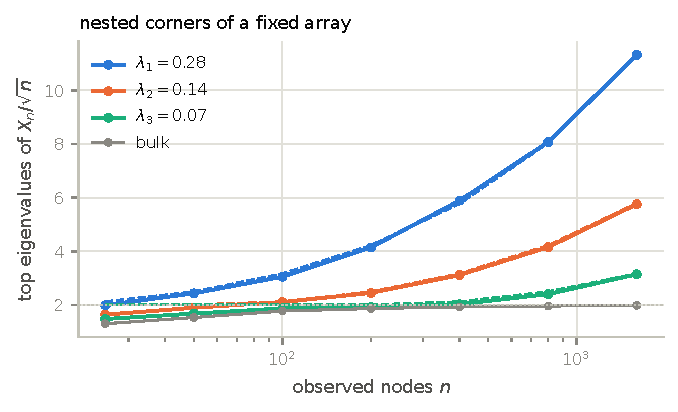
\includegraphics[width=0.54\textwidth]{figures/fig1_bbp.pdf}
\caption{Finite-$n$ calibration: top four eigenvalues of
$X_n/\sqrt n$ for nested corners of fixed arrays
($\blam=(0.28,0.14,0.07)$, $\sigma=1$; mean over 8 arrays generated
once at $n=1600$); dashed curves are $s_k+1/s_k$; the gray series is
the bulk edge. Supplement Figure~S1 shows the matching check of the
eigenvalue prediction at $n=2000$.}
\label{fig:bbp}
\end{figure}


\subsection{Level and power of the exact test}
\label{sec:exp-test}

Figure~\ref{fig:test}(a) measures the size of the hollow pipeline,
which Remark~\ref{rem:hollow} identifies as approximate: every matrix,
observed and replicate, is diagonal-zeroed before statistics are
computed. Across 250 null draws from spiked ensembles (spike count uniform on
$\{0,1,2,3\}$, magnitudes i.i.d.\ $U(1.2,3)$, Haar directions;
$n=120$, $B=99$; full specification in the released code), the conditional $p$-values of all
five statistics are uniform, and the Bonferroni-combined test rejects
at rate $0.068$ at nominal $0.05$ ($17/250$; Wilson 95\% interval
$[0.043,0.106]$): the approximation gap is within Monte Carlo error of
zero at this $n$. Because every applied matrix in this paper is a
finite-$T$ sample correlation or a transformed flow network, we also
measured the correlation pipeline, where the unit diagonal constrains
the matrix to the elliptope. For $T\times n$
panels of i.i.d.\ $N(0,1)$ entries with $n=120$, Fisher-$z$ sample
correlations, and the full battery ($R=100$, $B=99$), the combined test rejected at rate $0.060$ for $T=120$ and $0.040$
for $T=360$, every per-statistic rate at most $0.06$ (Supplement
Table~S1): the distortion from the elliptope constraint is within
Monte Carlo error of zero, consistent with the perturbation heuristic
of Remark~\ref{rem:hollow}.

The same ensemble calibrates the null models a practitioner might use
instead. Holding the rotatable truth fixed, a weight-permutation null
($B=99$) rejects the combined battery in $0.51$ of replicates at
nominal $0.05$, the miscalibration carried by exactly the summaries
applied fields report, clustering $0.57$ and strength-CV $0.42$; a
parametric bootstrap from the fitted spiked model attains $0.03$
combined with per-statistic rates up to $0.10$, roughly calibrated at
the price of fitting the model class and with no finite-sample
guarantee (Supplement Table~S2). The conditional test fits nothing and
is calibrated for any observed spectral shape, market modes and
Marchenko--Pastur bulks included; fitted or rewired generative
ensembles \citep{maslov2002specificity} test a different null and are
exact for none, quantified by the $0.51$ rejection rate above.

Figure~\ref{fig:test}(b) shows power against three exchangeable,
non-rotatable alternatives: a spike whose eigenvector interpolates from
delocalized to localized on $\lceil n^{2/3}\rceil$ coordinates; a
rank-2 graphon-Gaussian model with smooth bounded eigenfunctions
$\cos(\pi u),\cos(2\pi u)$; and heteroskedastic noise with log-normal
node variances. Localization is detected by the IPR statistic (power
$0.82$ at $\eta=1$, $0.74$ at $\eta=0.75$) and variance structure by
strength-CV (power $1.0$ from $\eta=0.2$). The graphon curve stays near
size over the whole range (rejection rates $0.02$ to $0.08$), and even
tripling the graphon signal (spikes $5.0,2.5$ at $n=200$) yields
combined power of only $0.56$. The theory explains this power gap: such a graphon differs from a
rotatable law only through the non-Gaussian geometry of its
eigenfunctions, the observable eigenvector is diluted to overlap
$\sqrt{1-\sigma^2/\theta^2}$ (Proposition~S2(ii)), and below the transition no consistent test exists against the
spherical-prior analogue (Corollary~S2); the cosine-direction curve is
the empirical counterpart. This battery, at these sizes,
has little power against weak smooth delocalized graphons; the
detectable departures are localization and scale heterogeneity, the
channels that reject on the real networks below.

\begin{figure}[t]
\centering
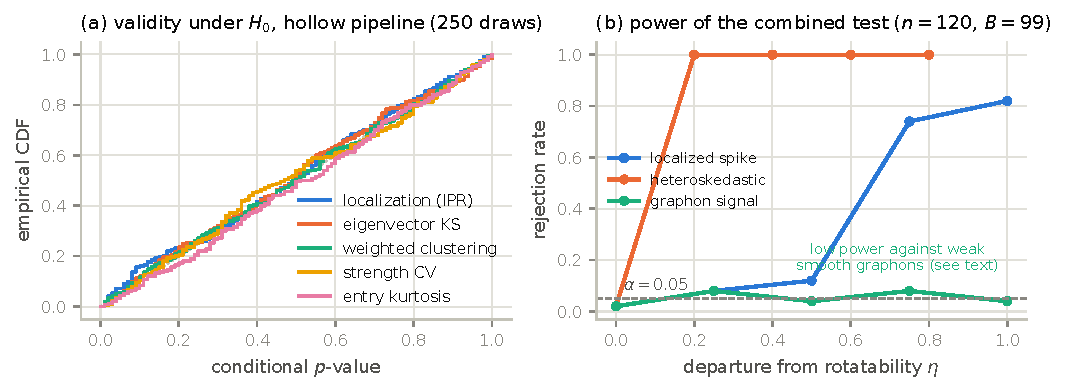
\includegraphics[width=0.92\textwidth]{figures/fig2_test.pdf}
\caption{The Haar-conditional rotation test. (a) Null $p$-value ECDFs
for the five statistics under the hollow pipeline (250 draws, $n=120$,
$B=99$); the diagonal is exact uniformity. (b) Power of the combined
battery against localized-spike, heteroskedastic, and smooth
graphon-Gaussian alternatives; the graphon alternative remains near
size (see text).}
\label{fig:test}
\end{figure}

\subsection{Real networks: which statistics reject, and what survives $G$}
\label{sec:exp-real}

\begin{table}[t]
\centering\small
\caption{Haar-conditional $p$-values (upper tail) on real networks,
before and after normal-scores Gaussianization $G$. HCP: group-average
functional connectome, Fisher-$z$, $n=200$, $B=499$. Air traffic:
$\log(1+\text{flow})$, $n=183$, $B=199$; the $G$ rows report ranges over
five tie-breaking seeds. S\&P~500: share of 28 rolling windows
(Fisher-$z$ correlations, $n=300$, $B=99$) with $p\le0.05$; modularity $p$-values were not computed per window (n/a here);
per-window modularity values enter the reconstruction study of
Section~\ref{sec:exp-cohort}. $p$-values near 1 indicate lower-tail
values (see text).}
\label{tab:real}
\begin{tabular}{llccccc}
\toprule
Network & version & IPR & clustering & modularity & strength CV & kurtosis\\
\midrule
HCP functional & raw & 0.004 & 0.836 & 1.000 & 1.000 & 0.002\\
 & after $G$ & 0.190 & 0.002 & 0.992 & 1.000 & 1.000\\
Air traffic & raw ($\log$) & 0.005 & 0.005 & 1.000 & 0.005 & 0.045\\
 & after $G$ & 0.005--0.020 & 0.005--0.010 & 1.000 & 0.005 & 1.000\\
S\&P 500 (share $p\le.05$) & raw & 0.25 & 0.75 & n/a & 0.00 & 0.25\\
 & after $G$ & 0.89 & 1.00 & n/a & 0.00 & 0.00\\
\bottomrule
\end{tabular}
\end{table}

Table~\ref{tab:real} and Figure~\ref{fig:real} report the test on
the three systems; all reject strict rotatability somewhere, as
expected, and the scientific content is in which statistics reject, in
the residuals, and in what survives $G$.

\emph{Human connectome.} The raw connectome rejects through localization
(IPR $p=0.004$, residual $z=+10.1$) and entry kurtosis ($p=0.002$,
$z=+89.7$), while the summaries network neuroscience most often reports
are not extreme in the upper tail: clustering sits inside its
conditional null ($p=0.836$, $z=-0.9$), and modularity and strength-CV
fall in the lower tail ($p\approx1$; $z=-16.6$ and $-10.3$). Given its
spectrum, the group-average connectome is less modular and less
strength-heterogeneous than a random rotation of that spectrum, and no
more clustered. After $G$ the localization rejection is no longer
significant ($p=0.190$) and kurtosis moves to the lower conditional tail
(upper-tail $p=1.000$), while a clustering
rejection appears ($p=0.002$): the marginal transform does not render every entry-level statistic consistent with the null. By the interpretation of Section~\ref{sec:diagnostic}, the localization
signal is consistent with a mainly tail-driven departure at this
resolution; group averaging can attenuate subject-level localization,
which the protocol of Section~\ref{sec:exp-cohort} measures on real
cohorts. This is one group-average matrix, a demonstration of the
method, with no claim about connectomes in general.

\emph{S\&P 500.} Across 28 rolling windows, strength-CV is uniformly
lower-tail (all windows at $p\ge0.95$) and kurtosis is lower-tail in
$0.68$: given spectra that include the market mode, the correlation
networks are more homogeneous in node strength than random rotations of
those spectra. Clustering rejects upper-tail in $0.75$ of raw windows
and all windows after $G$; IPR in $0.25$ raw and $0.89$ after $G$,
consistent with sector localization sharpened once the market-wide
scale is removed. These are per-window findings; windows overlap in
time.

\emph{Air traffic.} The log-flow network rejects through localization,
clustering, and strength-CV (all $p=0.005$), with kurtosis marginal
($p=0.045$) and modularity lower-tail. After $G$, repeated over five
tie-breaking seeds because most airport pairs have tied zero flows, kurtosis moves to the lower conditional tail (upper-tail $p=1.000$
at every seed) while
localization, clustering, and strength-CV persist at every seed (IPR
$p\in[0.005,0.020]$). The hub structure survives the marginal transform, consistent with
airline geography; the network is a positive control for the
diagnostic.

\begin{figure}[t]
\centering
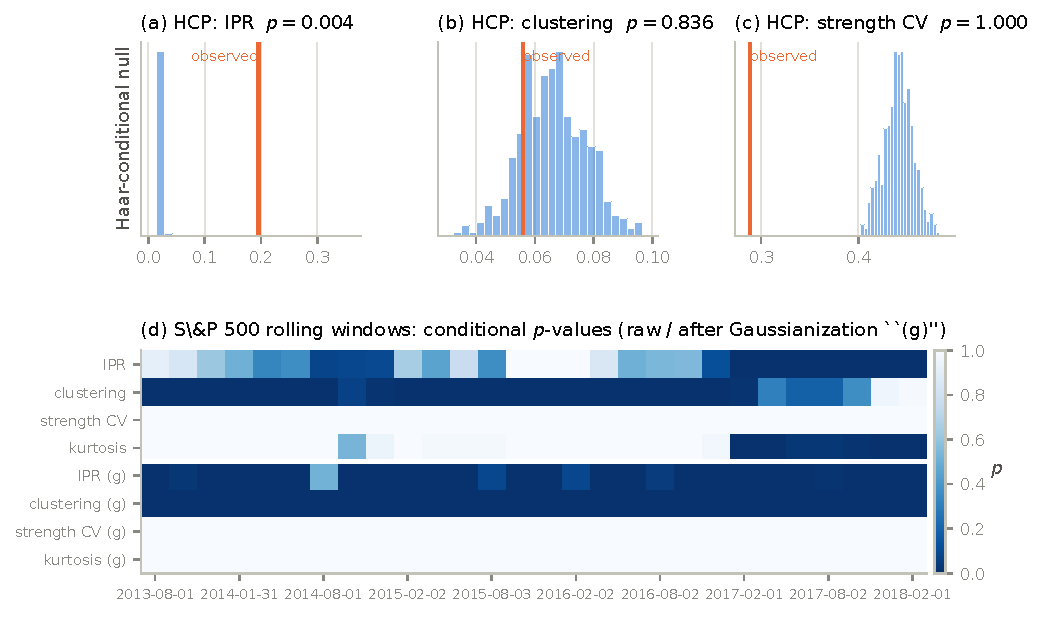
\includegraphics[width=0.92\textwidth]{figures/fig3_real.pdf}
\caption{Real networks. (a)--(c) HCP connectome: observed IPR,
clustering, and strength-CV against their Haar-conditional null
densities ($B=499$). (d) S\&P~500 rolling windows: conditional
$p$-values per window and statistic, raw and after Gaussianization.}
\label{fig:real}
\end{figure}

\subsection{Cohorts: sufficiency, residuals, and the protocol}
\label{sec:exp-cohort}

The cohort experiment implements the full protocol of
Sections~\ref{sec:sufficiency} and \ref{sec:test} on synthetic
cohorts calibrated to connectomic dimensions ($S=240$ subjects per
cohort, $n=200$, two groups). It validates the implementation of the
protocol and is evidence about the method, and about no real cohort;
the analysis environment could not reach the ABIDE bucket, and
Supplement Section~S4 specifies the identical pipeline, with fetch and
analysis code shipped, for the real data. Four feature sets enter
cross-validated logistic classifiers: spectral features, five
non-spectral summaries, the conditional residuals of those summaries
(Definition~\ref{def:residual}), and spectral plus summaries.

\emph{Cohort A: rotatable truth.} Both groups follow spiked
ensembles, the group difference planted in spike sizes. Spectral
features reach AUC $0.94\pm0.01$, raw summaries alone $0.89\pm0.01$
(marginally informative, as Remark~\ref{rem:scope} states), and adding
them to the spectrum gives no improvement ($0.93\pm0.01$). The
conditional residuals classify at chance ($0.46\pm0.02$): once each
subject's spectrum is conditioned out, the summaries carry no group
information. This is consistent with the parameter-free conditional
law of Corollary~S1; the marginal residual distribution can still vary
with the spectrum distribution, so chance-level classification is an
empirical finding here, and conditional-rank features give the exactly
invariant version. Per-subject
rotatability tests (Bonferroni at level $0.05$, 20 subjects per group)
reject for $0.00$ and $0.10$ of subjects, consistent with the level.

\emph{Cohort B: non-rotatable truth.} The spike-size distributions are
identical in the two groups, and group 1's leading eigenvector is
localized on 20 nodes. Spectral features classify at chance ($0.51\pm0.02$) while the
summaries and their residuals both reach AUC $1.00$: what the
summaries add is exactly a rotatability violation, and the residuals
isolate it. The per-subject test rejects
for $0.10$ of group-0 subjects and $1.00$ of group-1 subjects, so the
protocol of testing first and classifying on residuals second
identifies both the violation and the subjects carrying it.

\emph{S\&P 500 reconstruction.} Figure~\ref{fig:suff}(c) reports the
leave-one-out $R^2$ of predicting each summary of each rolling window
from six eigenvalue features of the same window: clustering $0.99$,
modularity $0.93$, kurtosis $0.82$, strength-CV $0.25$, IPR $0.03$. Two caveats: the windows overlap, so these are descriptive
within-sample associations, and the near-perfect reconstruction of
clustering is partly mechanical, since with one dominant market mode
clustering tracks the mean correlation level and hence $\lam_1$; the
result quantifies how much of each summary the spectrum determines,
the point of Corollary~S1, with no causal or predictive content.
The two summaries the eigenvalues fail to reconstruct, IPR and
strength-CV, are exactly the localization and scale statistics that
carry the conditional rejections in Table~\ref{tab:real}.

\begin{figure}[t]
\centering
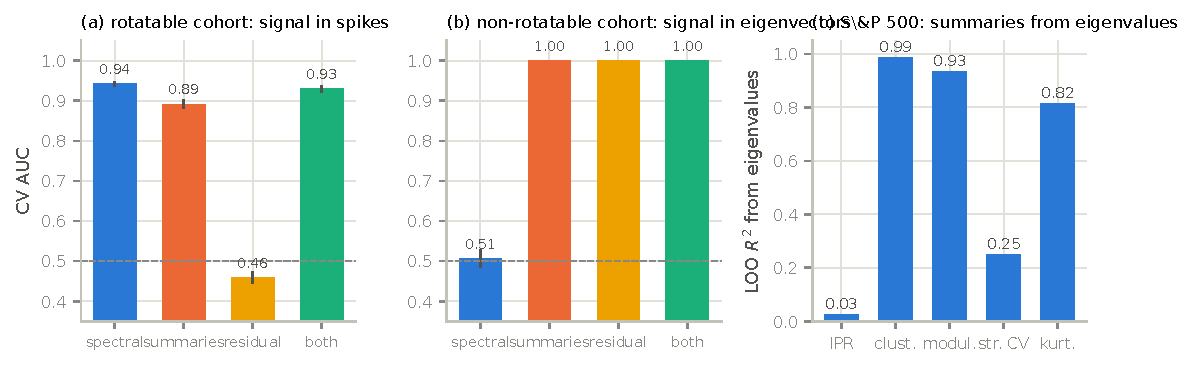
\includegraphics[width=0.92\textwidth]{figures/fig4_suff.pdf}
\caption{Cohorts and reconstruction. (a) Rotatable cohort: CV AUC on
spectral features, raw summaries, conditional residuals, and spectral
plus summaries; residuals are at chance. (b) Non-rotatable cohort
(localized eigenvector in group 1): spectral features are at chance;
summaries and residuals classify perfectly. (c) Leave-one-out $R^2$ of
predicting each summary of each S\&P~500 window from eigenvalue
features of the same window (descriptive; windows overlap).}
\label{fig:suff}
\end{figure}

\subsection{Nodewise attribution with exact familywise control}
\label{sec:exp-nodewise}

The nodewise protocol of Section~\ref{sec:test} was run on both real
networks, matching the Table~\ref{tab:real} pipelines
(Fisher-$z$ connectome, log-flow air network), with $\ell_i$ the
energy of node $i$ in the $K=10$ leading eigenvectors and $B=499$. On
the connectome, $8$ of $200$ parcels are flagged at familywise level
$0.05$ (global $p=0.008$), concentrated in two contiguous index
blocks of the Schaefer-200 ordering (parcels $12$--$13$ and
$102$--$113$): the aggregate IPR rejection of Table~\ref{tab:real}
is attributed to a short list of named parcels with an exact error
guarantee. On the air-traffic network, $8$ of $183$ airports are
flagged (global $p=0.006$): DEN, IAH, DFW, ORD, ATL, MSP, DTW, and
SLC, the major national hubs, so the attribution recovers the known
hub geography. In both cases the protocol turns an aggregate
localization rejection into a familywise-controlled list of nodes,
the output Section~\ref{sec:intro} argues applied work should
report.

\subsection{Heavy tails and the diagnostic}
\label{sec:exp-heavy}

Supplement Figure~S1(a) compares edge-weight tails: a spiked GOE draw
(Hill index $6.1$; fixed top-$5\%$ threshold, sensitivity analysis
deferred), the spiked $1.5$-stable law of
Theorem~\ref{thm:stable} (Hill $1.2$), and the raw air-traffic flows
(Hill $2.9$); the delocalized-spike stable control below has Hill
$1.6$. Supplement Figure~S1(b) applies the diagnostic of
Section~\ref{sec:diagnostic} to four networks; the synthetic ensembles
are tested as full matrices because their models specify diagonals, and
the hollow pipeline is used for the hollow air-traffic data (Supplement
Section~S3).

The Gaussian control rejects nothing before or after $G$. The
delocalized-spike stable control rejects kurtosis and IPR raw
($p=0.005$ each) and neither after $G$ (kurtosis $0.825$, IPR
$0.805$): a purely tail-driven violation, removed by the transform.
The Theorem~\ref{thm:stable} model rejects both raw ($p=0.005$);
after $G$ kurtosis moves to the lower conditional tail
(upper-tail $p=1.000$) while localization persists
($p=0.005$): heavy-tailed factors are genuinely $\ell_4$-localized,
the diagnostic reports it correctly, and the $p$-rotatable class with
nonzero spikes populates the persistent row. The
air-traffic network behaves like the factor model: kurtosis reverts
($p=1.000$ at all tie seeds) while localization persists
($p\le0.020$ at all seeds). The readout separates marginal,
transform-removable heaviness from persistent eigenvector structure; on
these data, air-traffic hubs are of the second kind.

\section{Discussion}
\label{sec:discussion}

\subsection{Summary}

Joint rotatability with sampling consistency characterizes the model
class as mixtures of spiked Gaussian orthogonal ensembles
(Theorem~\ref{thm:rep}), proved in full from
\citet[Theorem~5.1]{kallenberg1988some} with a unique canonical
parameterization. The spectrum is sufficient with Haar conditionals
(Theorem~\ref{thm:suff}), yielding the exact test for fully observed
matrices (Theorem~\ref{thm:test}), conditional residuals (Definition~\ref{def:residual}), consistency at every supercritical localized spike, with the
spherical-null trichotomy of Corollary~S2, the approximate-rotatability bound with its
preprocessing clause (Proposition~\ref{prop:robust}), the
statistic-level size guarantee for the zero-completion pipeline
(Proposition~\ref{prop:hollowrate}), and
Baik--Ben~Arous--P\'ech\'e calibration (Proposition~S2). An $\ell_p$ extension covers stable noise
(Theorem~\ref{thm:stable}), with completeness open
(Conjecture~\ref{conj:stable}). Empirically, the test is calibrated
under the pipeline used on data, rejects rotatability on all three real
systems in the directions the theory identifies, and the residuals
concentrate in eigenvector localization.

Rotatability is a sharp null hypothesis, and its value is the
direction of rejection: the statistics that reject, and their
conditional residuals, identify the structure in a network that its
spectrum does not determine. In the data analyzed here, several routinely tabulated summaries are
close to their Haar-conditional expectations given the spectrum while
localization is not; measuring residual eigenvector geometry, per node
and per component, appears to be the more informative target for
applied work.

\subsection{Limitations}

First, the theory is dense and real-valued; sparse weighted graphs need an
$\ell_p$-graphon-style thinning theory \citep{borgs2019lp,caron2017sparse}
that we do not provide, and binary graphs are outside the class. Second, exactness covers fully observed matrices only: hollow and
unit-diagonal data make exact rotatability degenerate, and the
total-variation gap in Proposition~\ref{prop:robust} equals one for
them (Remark~\ref{rem:hollow}). Proposition~\ref{prop:hollowrate} supplies the statistic-level
replacement, with rate $n^{-1/4}(\log n)^{1/2}$ under Lipschitz and
bounded-density hypotheses that are stated, not verified, for the
specific battery, and the measured sizes are within Monte
Carlo error of nominal; an exact conditional theory on the
fixed-diagonal isospectral manifold, and an analogous bound for the
finite-$T$ correlation step, remain open.
Third, the $p<2$ theory is asymmetric: the construction and invariance are
proved, completeness is conjectured, and without a $p$-analogue of the
Haar frame there is no exact conditional test at $p<2$; the Gaussianization
diagnostic tests a surrogate null, and, because $\SaS$ factors are
themselves localized, it does not separate the $p$-rotatable class from
structural localization. Fourth, the proved power theory is limited:
consistency holds for supercritical $\ell_4$-nondegenerate spikes
(Proposition~S3), the battery has low power against weak
smooth delocalized graphon alternatives at the sample sizes studied, and
no optimality claims are made. Fifth, the cohort study is synthetic, calibrated to connectomic
dimensions and labeled as such; the group-average HCP connectome is a
single matrix; the S\&P~500 windows overlap in time, so cross-window
$R^2$ values are descriptive only. Sixth, Monte Carlo settings are
moderate ($B$ between $99$ and $499$, $250$ null replicates for the
level study); exactness does not depend on $B$, but power and the
precision of reported rates do.

\subsection{Future work}

In order of priority: a subject-level replication on real cohorts,
for which Supplement Section~S4 specifies the ABIDE protocol and the
fetch and analysis code ships with the paper; exact conditional sampling on the isospectral manifold with fixed
diagonal, and the extension of Proposition~\ref{prop:hollowrate} to
the finite-$T$ correlation step, which together would close the
exactness gap of Remark~\ref{rem:hollow}; models rotatable conditionally on a
low-dimensional non-rotatable component, such as an anatomical template
plus rotatable deviations; optimal and adaptive tests against spiked-graphon alternatives
\citep{onatski2013asymptotic,perry2018optimality}, minimax estimation of $\blam$, fluctuation theory for the plug-in
estimators, and the extension of the nodewise protocol from
familywise to false-discovery control; joint invariance for
families of networks, where between-network eigenspace alignment is
the new non-spectral information; completing the heavy-tailed theory, Conjecture
\ref{conj:stable}, the aggregation-scaling estimator of $p$, and a
calibrated test at $p<2$; and sparse and directed extensions, the
latter via the unitary-invariant Hermitian theory
\citep{olshanski1996ergodic,vershik2002}.

Under joint rotatability the eigenvalues carry all information about the
model, exactly and at every $n$. Where data reject the symmetry, the
rejecting statistics and their conditional residuals locate the structure
that the spectrum does not determine; making that decomposition exact and
routinely computable is the contribution of this paper.


\ifnum\blind=0
\section*{Acknowledgments}
[Personal and funding acknowledgments; unblinded version only.]

\section*{Disclosure of generative AI use}
In accordance with the Taylor \& Francis policy on artificial
intelligence, the authors disclose that a generative AI assistant
(Claude, Anthropic; [record the model version used]) was used, under
author direction, to draft and revise manuscript text, to write and
refactor the simulation and analysis code released with the paper, and
to draft the proof of Proposition~\ref{prop:robust}. The authors
specified the mathematical content, verified all statements and proofs,
re-ran all released code, and take full responsibility for the content.
The tool was not used to create or alter research data.
\fi

% Reference-list spacing: the official ASA/T&F template governs final
% spacing; 1.5 here keeps this stand-in build within the page ceiling.
\begin{spacing}{1.0}\small\setlength{\bibsep}{2pt}
\bibliographystyle{apalike}
\bibliography{refs}
\end{spacing}

\end{document}
